\subsubsection{Characteristics}
A typical delta pattern has the following characteristics:

\begin{itemize}

\item The constellation contains a total of \textit{T} satellites evenly spaced in each of the \textit{P} orbital planes. All planes have the same number of satellites, defined as \textit{S}, equally distributed. Thus:
\begin{equation}
T = SP
\end{equation}
\begin{equation}
\Delta\varphi=\frac{2\pi}{S}
\end{equation}
Where $\Delta\varphi$ is the angle between satellites in the same plane.

\item All orbits have equal inclinations $\delta$ to a reference plane. If this plane is the Equator (it usually is), then the inclination $\delta$ equals the orbital parameter inclination \textit{i} \cite{Walker1971}.
\begin{figure}[h!]
\centerline{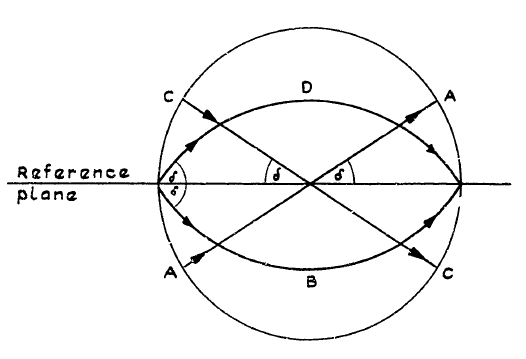
\includegraphics[scale=0.5]{Full/Deltapattern.png}}
\caption{Definition of the inclination $\delta$. Extracted from \cite{Walker1971}}
\label{fig:delta pattern}
\end{figure} 

\item The ascending nodes of the orbits are equally spaced across the full $2\pi$ (360$^{\circ}$ of longitude) at intervals of:
\begin{equation}
\Delta\Omega=\frac{2\pi}{P}
\end{equation}

\item The position of the satellites in different orbital planes is measured through the factor \textit{F}. When a satellite is at its ascending node, a satellite in the most easterly adjacent plane has covered a relative phase difference \textit{F}. The real phase difference is defined as:
\begin{equation}
\Delta\Phi=F\frac{2\pi}{P}
\end{equation}
In order to have the same phase difference between all orbital planes, \textit{F} is defined as an integer, which may have any value from 0 to (P-1).

\end{itemize}

\begin{figure}[h!]
\centerline{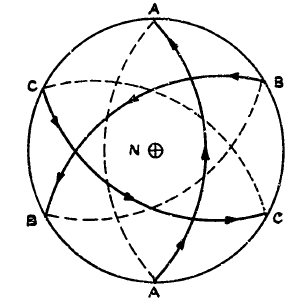
\includegraphics[scale=0.75]{Full/walkerdeltaplanta.png}}
\caption{Delta pattern as seen from the North Pole. Extracted from \cite{Walker1977}}
\label{fig:delta pattern North Pole}
\end{figure}

With these characteristics, delta constellations are more complex than polar constellations. Because of the inclination of the orbits, the ascending and descending planes and the coverage of the satellites continuously overlap. This characteristic is a constraint on intersatellite networking because the relative velocities between satellites in different orbital planes are larger than in a polar constellation. Consequently, tracking requirements and Doppler shift are increased \cite{Wood1940}.

\begin{figure}[h!]
\centerline{\includegraphics[scale=0.75]{Full/wdperspectiva}}
\caption{Delta pattern 65$^{\circ}$: 30/6/1}
\label{fig:delta pattern notation}
\end{figure}

\subsubsection{Notation}
J.G. Walker developed a notation to define this constellations with only 4 parameters \cite{Walker1977}:
\begin{equation*}
i: T/P/F
\end{equation*}
Since all satellites are placed at the same altitude, with these notation the shape of the pattern is completely determined. However, to determine all the orbital parameters it is necessary to know the radius of the orbits.

\subsubsection{Coverage}
The previous section has shown that in polar orbits the coverage of the constellation could be determined with the streets of coverage method. On the other hand, in delta patterns it is necessary to study each configuration to verify its coverage. J.G. Walker determined that delta patterns gave better coverage than polar orbits, but not substantially better in the case of single coverage. This kind of patterns are more useful for double or triple coverage constellations, as it can be seen in Figure \ref{fig:Walker vs. polar}. However, his calculations were for a low number of satellites, so it is necessary to compute new results for the number of satellites of the Astrea constellation.
\begin{figure}[h]
\centerline{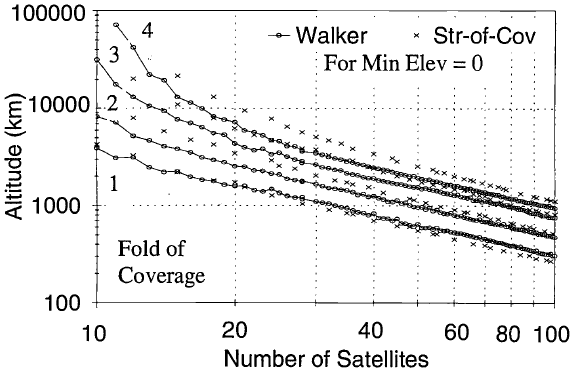
\includegraphics[scale=0.75]{Full/foldofcoverage.png}}
\caption{Minimum altitude for continuous global coverage. Comparison between polar patterns and Walker delta patterns. Extracted from \cite{Chobotov2002}}
\label{fig:Walker vs. polar}
\end{figure}